% Options for packages loaded elsewhere
\PassOptionsToPackage{unicode}{hyperref}
\PassOptionsToPackage{hyphens}{url}
%
\documentclass[
  english,
  man]{apa6}
\usepackage{lmodern}
\usepackage{amssymb,amsmath}
\usepackage{ifxetex,ifluatex}
\ifnum 0\ifxetex 1\fi\ifluatex 1\fi=0 % if pdftex
  \usepackage[T1]{fontenc}
  \usepackage[utf8]{inputenc}
  \usepackage{textcomp} % provide euro and other symbols
\else % if luatex or xetex
  \usepackage{unicode-math}
  \defaultfontfeatures{Scale=MatchLowercase}
  \defaultfontfeatures[\rmfamily]{Ligatures=TeX,Scale=1}
\fi
% Use upquote if available, for straight quotes in verbatim environments
\IfFileExists{upquote.sty}{\usepackage{upquote}}{}
\IfFileExists{microtype.sty}{% use microtype if available
  \usepackage[]{microtype}
  \UseMicrotypeSet[protrusion]{basicmath} % disable protrusion for tt fonts
}{}
\makeatletter
\@ifundefined{KOMAClassName}{% if non-KOMA class
  \IfFileExists{parskip.sty}{%
    \usepackage{parskip}
  }{% else
    \setlength{\parindent}{0pt}
    \setlength{\parskip}{6pt plus 2pt minus 1pt}}
}{% if KOMA class
  \KOMAoptions{parskip=half}}
\makeatother
\usepackage{xcolor}
\IfFileExists{xurl.sty}{\usepackage{xurl}}{} % add URL line breaks if available
\IfFileExists{bookmark.sty}{\usepackage{bookmark}}{\usepackage{hyperref}}
\hypersetup{
  pdftitle={Simulation checks},
  pdfauthor={Marie Delacre1, Daniel Lakens2, Christophe Ley3, Limin Liu3, \& Christophe Leys1},
  hidelinks,
  pdfcreator={LaTeX via pandoc}}
\urlstyle{same} % disable monospaced font for URLs
\usepackage{graphicx,grffile}
\makeatletter
\def\maxwidth{\ifdim\Gin@nat@width>\linewidth\linewidth\else\Gin@nat@width\fi}
\def\maxheight{\ifdim\Gin@nat@height>\textheight\textheight\else\Gin@nat@height\fi}
\makeatother
% Scale images if necessary, so that they will not overflow the page
% margins by default, and it is still possible to overwrite the defaults
% using explicit options in \includegraphics[width, height, ...]{}
\setkeys{Gin}{width=\maxwidth,height=\maxheight,keepaspectratio}
% Set default figure placement to htbp
\makeatletter
\def\fps@figure{htbp}
\makeatother
\setlength{\emergencystretch}{3em} % prevent overfull lines
\providecommand{\tightlist}{%
  \setlength{\itemsep}{0pt}\setlength{\parskip}{0pt}}
\setcounter{secnumdepth}{-\maxdimen} % remove section numbering
% Make \paragraph and \subparagraph free-standing
\ifx\paragraph\undefined\else
  \let\oldparagraph\paragraph
  \renewcommand{\paragraph}[1]{\oldparagraph{#1}\mbox{}}
\fi
\ifx\subparagraph\undefined\else
  \let\oldsubparagraph\subparagraph
  \renewcommand{\subparagraph}[1]{\oldsubparagraph{#1}\mbox{}}
\fi
% Manuscript styling
\usepackage{upgreek}
\captionsetup{font=singlespacing,justification=justified}

% Table formatting
\usepackage{longtable}
\usepackage{lscape}
% \usepackage[counterclockwise]{rotating}   % Landscape page setup for large tables
\usepackage{multirow}		% Table styling
\usepackage{tabularx}		% Control Column width
\usepackage[flushleft]{threeparttable}	% Allows for three part tables with a specified notes section
\usepackage{threeparttablex}            % Lets threeparttable work with longtable

% Create new environments so endfloat can handle them
% \newenvironment{ltable}
%   {\begin{landscape}\begin{center}\begin{threeparttable}}
%   {\end{threeparttable}\end{center}\end{landscape}}
\newenvironment{lltable}{\begin{landscape}\begin{center}\begin{ThreePartTable}}{\end{ThreePartTable}\end{center}\end{landscape}}

% Enables adjusting longtable caption width to table width
% Solution found at http://golatex.de/longtable-mit-caption-so-breit-wie-die-tabelle-t15767.html
\makeatletter
\newcommand\LastLTentrywidth{1em}
\newlength\longtablewidth
\setlength{\longtablewidth}{1in}
\newcommand{\getlongtablewidth}{\begingroup \ifcsname LT@\roman{LT@tables}\endcsname \global\longtablewidth=0pt \renewcommand{\LT@entry}[2]{\global\advance\longtablewidth by ##2\relax\gdef\LastLTentrywidth{##2}}\@nameuse{LT@\roman{LT@tables}} \fi \endgroup}

% \setlength{\parindent}{0.5in}
% \setlength{\parskip}{0pt plus 0pt minus 0pt}

% Overwrite redefinition of paragraph and subparagraph by the default LaTeX template
% See https://github.com/crsh/papaja/issues/292
\makeatletter
\renewcommand{\paragraph}{\@startsection{paragraph}{4}{\parindent}%
  {0\baselineskip \@plus 0.2ex \@minus 0.2ex}%
  {-1em}%
  {\normalfont\normalsize\bfseries\itshape\typesectitle}}

\renewcommand{\subparagraph}[1]{\@startsection{subparagraph}{5}{1em}%
  {0\baselineskip \@plus 0.2ex \@minus 0.2ex}%
  {-\z@\relax}%
  {\normalfont\normalsize\itshape\hspace{\parindent}{#1}\textit{\addperi}}{\relax}}
\makeatother

% \usepackage{etoolbox}
\makeatletter
\patchcmd{\HyOrg@maketitle}
  {\section{\normalfont\normalsize\abstractname}}
  {\section*{\normalfont\normalsize\abstractname}}
  {}{\typeout{Failed to patch abstract.}}
\patchcmd{\HyOrg@maketitle}
  {\section{\protect\normalfont{\@title}}}
  {\section*{\protect\normalfont{\@title}}}
  {}{\typeout{Failed to patch title.}}
\makeatother
\shorttitle{Simulation checks}
\keywords{\newline\indent Word count: 501 words}
\DeclareDelayedFloatFlavor{ThreePartTable}{table}
\DeclareDelayedFloatFlavor{lltable}{table}
\DeclareDelayedFloatFlavor*{longtable}{table}
\makeatletter
\renewcommand{\efloat@iwrite}[1]{\immediate\expandafter\protected@write\csname efloat@post#1\endcsname{}}
\makeatother
\usepackage{lineno}

\linenumbers
\usepackage{csquotes}
\usepackage{rotating}
\DeclareDelayedFloatFlavor{sidewaysfigure}{figure}
\usepackage{lscape}
\newcommand{\blandscape}{\begin{landscape}}
\newcommand{\elandscape}{\end{landscape}}
\ifxetex
  % Load polyglossia as late as possible: uses bidi with RTL langages (e.g. Hebrew, Arabic)
  \usepackage{polyglossia}
  \setmainlanguage[]{english}
\else
  \usepackage[shorthands=off,main=english]{babel}
\fi

\title{Simulation checks}
\author{Marie Delacre\textsuperscript{1}, Daniel Lakens\textsuperscript{2}, Christophe Ley\textsuperscript{3}, Limin Liu\textsuperscript{3}, \& Christophe Leys\textsuperscript{1}}
\date{}


\authornote{

Correspondence concerning this article should be addressed to Marie Delacre, CP191, avenue F.D. Roosevelt 50, 1050 Bruxelles. E-mail: \href{mailto:marie.delacre@ulb.be}{\nolinkurl{marie.delacre@ulb.be}}

}

\affiliation{\vspace{0.5cm}\textsuperscript{1} Université Libre de Bruxelles, Service of Analysis of the Data (SAD), Bruxelles, Belgium\\\textsuperscript{2} Eindhoven University of Technology, Human Technology Interaction Group, Eindhoven, the Netherlands\\\textsuperscript{3} Universiteit Gent, Department of Applied Mathematics, Computer Science and Statistics, Gent, Belgium}

\begin{document}
\maketitle

\hypertarget{supplemental-material-2}{%
\section{Supplemental Material 2}\label{supplemental-material-2}}

In order to insure the reliability of our calculation method, for all scenarios where \(G_1=G_2=0\), we compared empirical means and variances of all estimators (i.e.~means and variances of all estimates) with theoretical means and variances (i.e.~expected means and variances, computed based on equations in Tables 1, 2 and 3 in the main article). Because we can draw exactly the same conclusions for \textbf{biased} (Cohen's \(d_s\), Glass's \(d_s\) using either \(S_1\) or \(S_2\) as standardizer, Shieh's \(d_s\) and Cohen's \(d^*_s\)) and \textbf{unbiased} (Hedges' \(g_s\), Glass's \(g_s\) using either \(S_1\) or \(S_2\) as standardizer, Shieh's \(g_s\) and Hedges' \(g^*_s\)) estimators, we will simultaneously present results for both categories of estimators. Results will be subdivided into 4 conditions:\\
- When population variances and sample sizes are equal across groups (condition a; see Figures A2.1 and A2.5 for respectively biased and unbiased estimators);\\
- When population variances are equal across groups and sample sizes are unequal (condition b; see Figures A2.2 and A2.6 for respectively biased and unbiased estimators);\\
- When population variances are unequal across groups and sample sizes are equal (condition c; see Figures A2.3 and A2.7 for respectively biased and unbiased estimators);\\
- When population variances and sample sizes are unequal across groups (condition d; see Figures A2.4 and A2.8 for respectively biased and unbiased estimators).

Because the equations of theoretical means and variances of Cohen's \(d_s\) and Hedges' \(g_s\) rely on the assumption of normality and equality of population variances, we expect empirical and theoretical parameters to be very close only in conditions a and b. For all other estimators, the equations of theoretical means and variances rely solely on the assumption of normality and therefore, we expect empirical and theoretical parameters to be very close in all conditions.

On average, empirical means (and variances) of all estimators are very close to theoretical expectations when population variances are equal across groups, with equal sample sizes (condition a; see Tables A2.1 and A2.5) or unequal sample sizes (condition b; see Tables A2.2 and A2.6).

When population variances are unequal across groups (conditions c and d; see Tables A2.3, A2.4, A2.7 and A2.8), empirical means (and variances) of Cohen's \(d^*_s\) (Hedges' \(g^*_s\)) and Shieh's \(d_s\) (Shieh's \(g_s\)) are still very close to theoretical expectations. Regarding Glass's \(d_s\) (Glass's \(g_s\)), on average, while empirical variances remain very close to theoretical expectations, one observes larger departures between empirical and theoretical means when using \(S_2\) as standardizer. However, when looking at details in results for each scenario (see \enquote{biased estimator\_condition C.xlsx}, \enquote{biased estimator\_condition D.xlsx}, \enquote{unbiased estimator\_condition C.xlsx} and \enquote{unbiased estimator\_condition C.xlsx} in Supplemental Material 2), one notices that the larger the population effect size, the larger the departure between empirical and theoretical means, and that relative to the population effect size, departures between empirical and theoretical means are always very small. On the other hand, both empirical bias and variance of Cohen's \(d_s\) (Hedges' \(g_s\)) highly depart from theoretical expectations, even when looking at relative departures to the population effect size, especially when sample sizes are unequal across groups (condition d; see Table A2.4 and A2.8), which is not surprising, as Cohen's \(d_s\) (Hedges' \(g_s\)) relies on the equality of population variances assumption.

\begin{sidewaysfigure}

{\centering 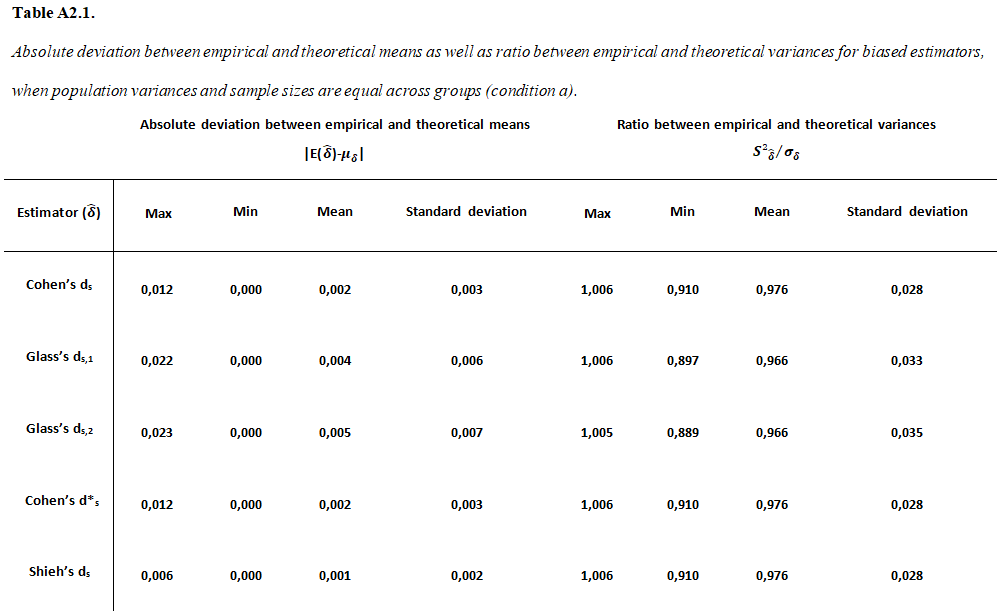
\includegraphics[width=12.53in]{D:/Documents/Github_projects/Effect-sizes/Supplemental Material 2/Files/Png tables/Table A2.1} 

}

\end{sidewaysfigure}

\begin{sidewaysfigure}

{\centering 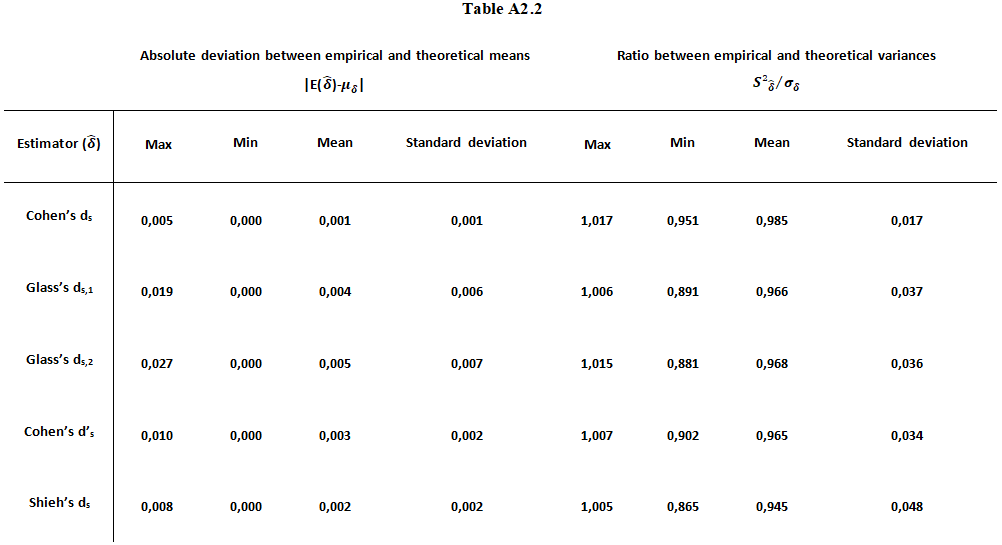
\includegraphics[width=12.46in]{D:/Documents/Github_projects/Effect-sizes/Supplemental Material 2/Files/Png tables/Table A2.2} 

}

\end{sidewaysfigure}

\begin{sidewaysfigure}

{\centering 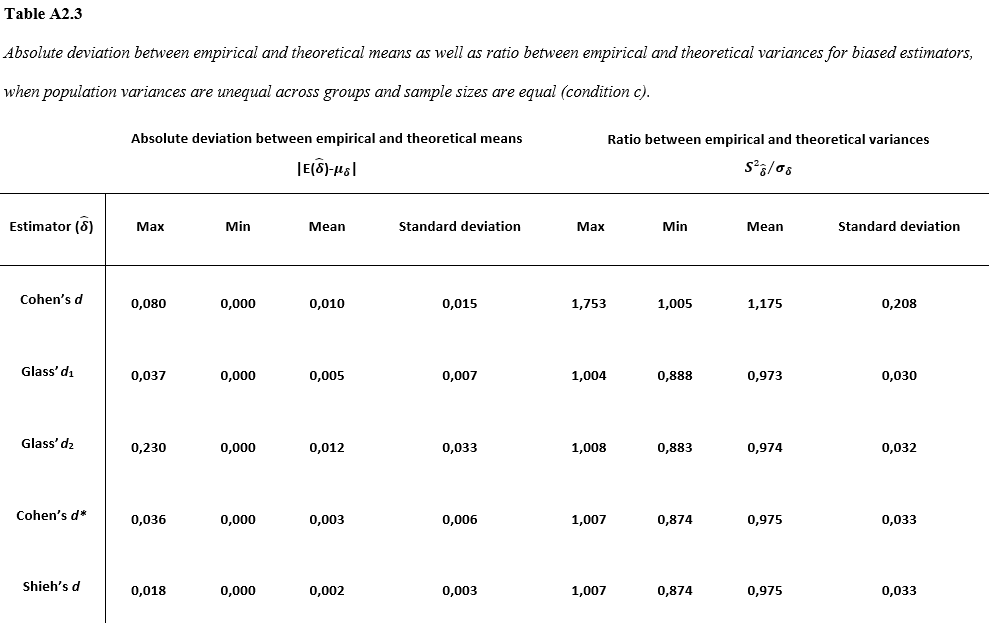
\includegraphics[width=12.47in]{D:/Documents/Github_projects/Effect-sizes/Supplemental Material 2/Files/Png tables/Table A2.3} 

}

\end{sidewaysfigure}

\begin{sidewaysfigure}

{\centering 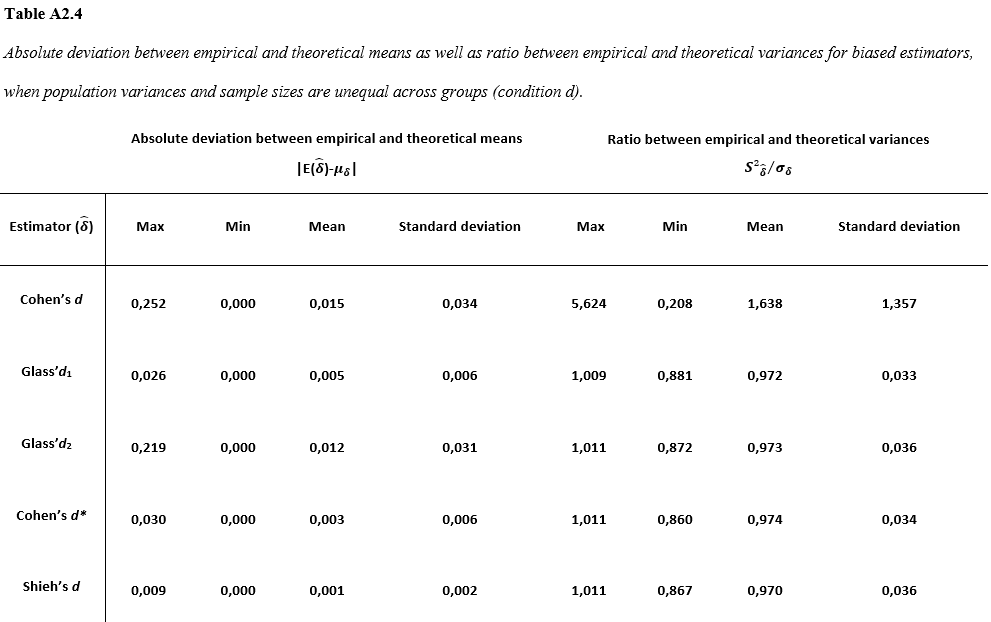
\includegraphics[width=12.51in]{D:/Documents/Github_projects/Effect-sizes/Supplemental Material 2/Files/Png tables/Table A2.4} 

}

\end{sidewaysfigure}

\begin{sidewaysfigure}

{\centering 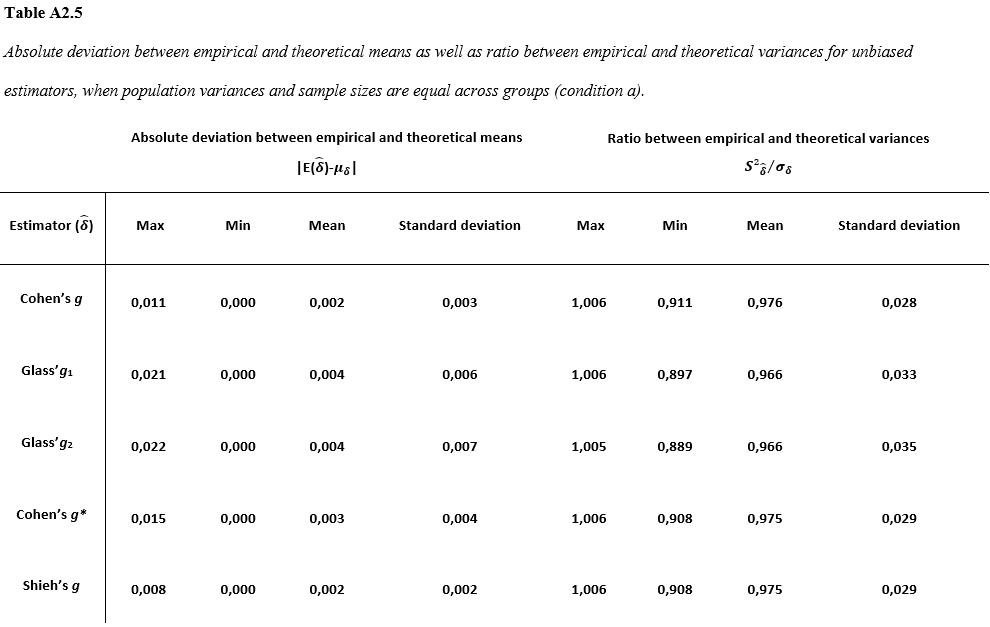
\includegraphics[width=12.49in]{D:/Documents/Github_projects/Effect-sizes/Supplemental Material 2/Files/Png tables/Table A2.5} 

}

\end{sidewaysfigure}

\begin{sidewaysfigure}

{\centering 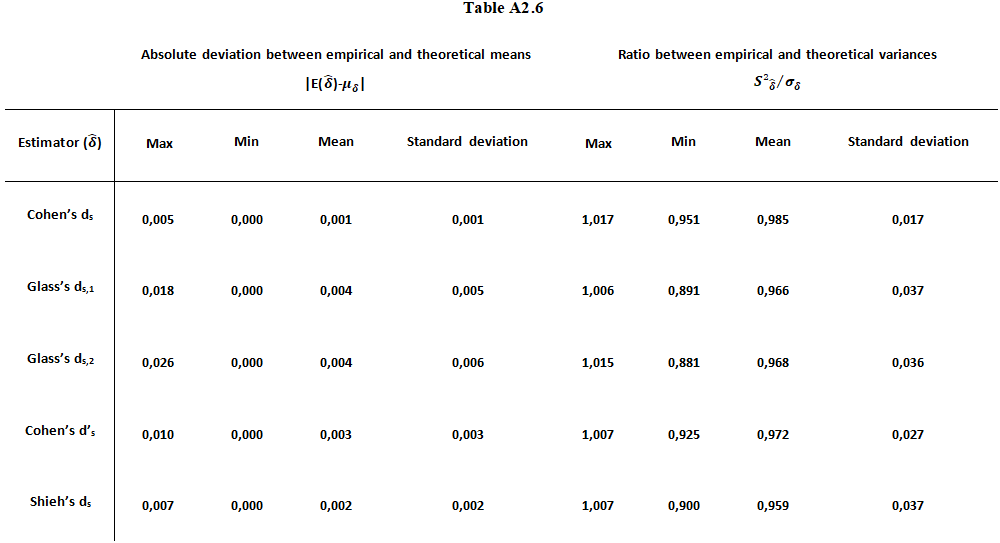
\includegraphics[width=12.5in]{D:/Documents/Github_projects/Effect-sizes/Supplemental Material 2/Files/Png tables/Table A2.6} 

}

\end{sidewaysfigure}

\begin{sidewaysfigure}

{\centering 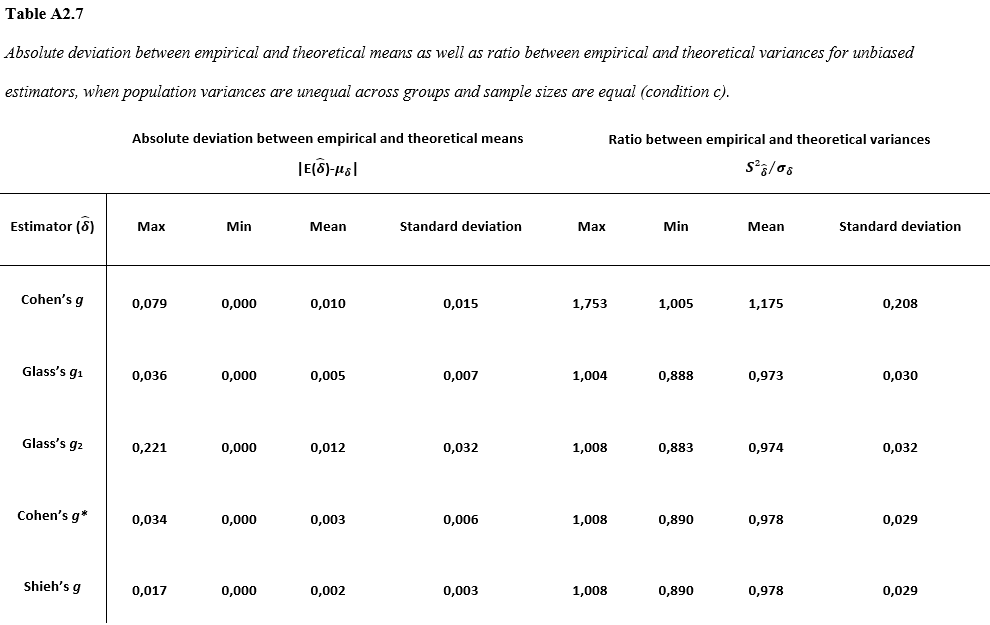
\includegraphics[width=12.49in]{D:/Documents/Github_projects/Effect-sizes/Supplemental Material 2/Files/Png tables/Table A2.7} 

}

\end{sidewaysfigure}

\begin{sidewaysfigure}

{\centering 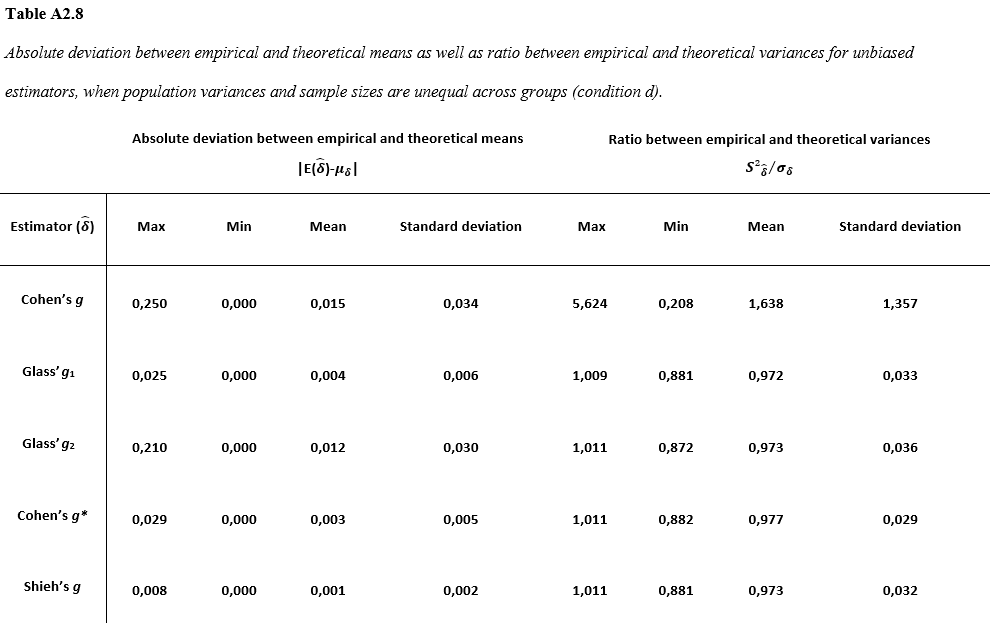
\includegraphics[width=12.49in]{D:/Documents/Github_projects/Effect-sizes/Supplemental Material 2/Files/Png tables/Table A2.8} 

}

\end{sidewaysfigure}


\end{document}
